% !TEX TS-program = pdflatex
% !TEX encoding = UTF-8 Unicode

\documentclass{beamer}



\mode<presentation>
{
  \usetheme{Boadilla}
}


\usepackage[english]{babel}

\usepackage[utf8]{inputenc}
\usepackage{times}
\usepackage[T1]{fontenc}
\usepackage{graphicx}
\graphicspath{ {./photo/} }

\title[Strojno učenje] 
{Strojno učenje}

\author[Križnar Karel, Dobravec Blaž]
{Križnar Karel \and Dobravec Blaž}


\institute
{
  Praktična matematika\\
  Fakulteta za matematiko in fiziko
}
\date
{17.1.2019 / Seminar}

%fotografija
\pgfdeclareimage[height=1 cm]{university-logo}{photo/logo}
\logo{\pgfuseimage{university-logo}}





\beamerdefaultoverlayspecification{<+->}


\begin{document}

\begin{frame}
  \titlepage
\end{frame}





\section{Introduction}

\subsection[uvod]{Uvod}

\begin{frame}
\frametitle[alignment=center]{Splošno} % ne delaaaaaa :(
  \begin{itemize}
  \item
    Kaj sploh je strojno učenje?
  \item
    Kje se strojno učenje uporablja?
  \item
    Umetna inteligenca = strojno učenje?
  \end{itemize}
\bigskip
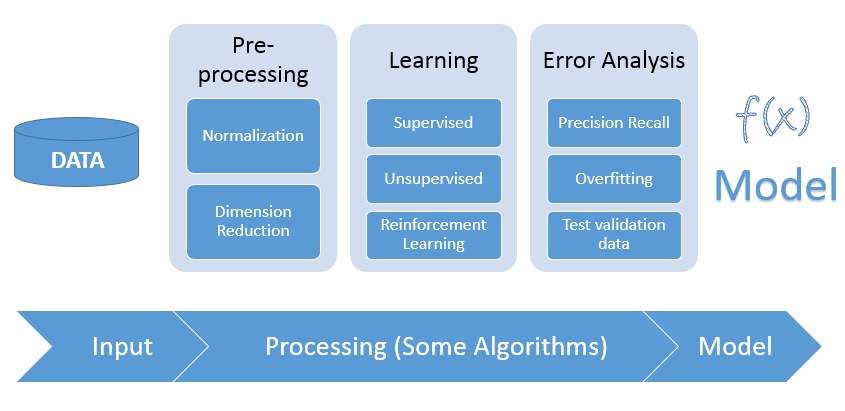
\includegraphics[scale = 0.3]{photo/ucenje_proces}
\end{frame}

\begin{frame}{Tipi strojnega učenja}
\bigskip
  Poznamo različne tipe strojnega učenja: \smallskip

  \begin{itemize}
  \item 
    \textbf{Nadzorovano učenje} $\rightarrow Algoritem $\texttt{ uči}  stroj na podlagi podanih parov vhodnih in željenih podatkov. Pri tem željene rezultate določa človek.
  \item 
     \textbf{Nenadzorovano učenje} $\rightarrow  Algoritem $\texttt{ razdeli} podatke v več skupin, ki imajo svoje značilnosti. Značilnosti algoritem izlušči iz vhodnih podatkov, brez pomoči človeka.
  \item 
     \textbf{Vzpodbujevalno učenje} $\rightarrow Algoritem $\texttt{ se priuči} vedenje oziroma optimizacijo vedenja na podlagi povratne informacije prek nagrajevanja oz. kaznovanja.
  \end{itemize}
\end{frame}


\begin{frame}{Uporaba vsakega od tipov}
  \begin{itemize}
  \item
   Nadzorovano učenje
	\begin{itemize}
  	\item
   	  Napovedovanje vremena
  	\item
   	  \alert{Klasifikacija fotografij}
  	\item
   	  Ocenjevanje nevarnosti
	\end{itemize}
  \item
  Nenadzorovano učenje
    	\begin{itemize}
  	\item
   	  Medicinske raziskave
  	\item
   	  \alert{Ciljno in lokacijsko oglaševanje}
	\end{itemize}
  \item
   Vzpodbujevalno učenje
 	\begin{itemize}
  	\item
   	  Računalniške igre
  	\item
   	  \alert{Navigacija robotov}
  	\item
   	  Napovedovanje delnic
	\end{itemize}
  \end{itemize}
\end{frame}


\subsection{Prepoznavanje števil}

\begin{frame}{Make Titles Informative.}
\end{frame}

\begin{frame}{Make Titles Informative.}
\end{frame}





\section*{Summary}

\begin{frame}{Summary}

  % Keep the summary *very short*.
  \begin{itemize}
  \item
    The \alert{first main message} of your talk in one or two lines.
  \item
    The \alert{second main message} of your talk in one or two lines.
  \item
    Perhaps a \alert{third message}, but not more than that.
  \end{itemize}
  
  % The following outlook is optional.
  \vskip0pt plus.5fill
  \begin{itemize}
  \item
    Outlook
    \begin{itemize}
    \item
      Something you haven't solved.
    \item
      Something else you haven't solved.
    \end{itemize}
  \end{itemize}
\end{frame}


\end{document}


